\section{What this thesis is about}

\begin{marginfigure}
\centering
\[\resizebox{0.5\textwidth}{!}{\tikzfig{intro/model}}\]
\caption{Let's say that \textbf\emph{{the meaning of text is how it updates a model.}} So we start with some model of the way things are, modelled as data on a wire.}
\end{marginfigure}

\begin{marginfigure}
\centering
\[\resizebox{0.6\textwidth}{!}{\tikzfig{intro/model2}}\]
\caption{Text updates that model; like a gate updates the data on a wire.}
\end{marginfigure}

\begin{marginfigure}
\centering
\[\resizebox{0.7\textwidth}{!}{\tikzfig{intro/model3}}\]
\caption{Text is made of sentences; like a circuit is made of gates and wires.}
\end{marginfigure}

\begin{marginfigure}
\centering
\[\resizebox{0.8\textwidth}{!}{\tikzfig{intro/model4}}\]
\caption{Let's say that \textbf{\emph{The meaning of a sentence is how it updates the meanings of its parts.}} As a first approximation, let's say that the \emph{parts} of a sentence are the nouns it contains or refers to. Noun data is carried by wires. Collections of nouns are related by gates, which play the roles of verbs and adjectives.}
\end{marginfigure}

\begin{marginfigure}
\centering
\[\resizebox{0.9\textwidth}{!}{\tikzfig{intro/model5}}\]
\caption{Gates can be related by higher order gates, which play the roles of adverbs, adpositions, and conjunctions; anything that modifies the data of first order gates like verbs.}
\end{marginfigure}

\begin{marginfigure}
\centering
\[\resizebox{\textwidth}{!}{\tikzfig{intro/model6}}\]
\caption{In practice, higher order gates may be implemented as gates that modify parameters of other gates. Parameters are depicted as additional inputs to gates.}
\end{marginfigure}

\begin{marginfigure}
\centering
\[placeholder\]
\caption{Grammar, and \emph{function words} -- words that operate on meanings -- are absorbed by the geometry of the diagram.}
\end{marginfigure}

\newthought{This thesis is about mathematically approximating natural language text using string diagrams.}

Text diagrams are compositional blueprints that may be instantiated by classical or quantum computers. Since we know how grammar composes meanings in language, we can quotient out grammar using these formal diagrams. In terms of potential practical value, this process turns big black boxes into composites of small black boxes, which is a happy middle ground for humans and computers: smaller pieces for machines to learn representations for, and easy-to-reckon representations for humans. In terms of theoretical value for formal linguistics, the mathematics of string diagrams -- applied category theory -- allows us to unify different views of syntax and expand the reach of what can be formalised. Enjoy a sideshow in the margins.

\newthought{\textbf{Point of information:} What do you mean by natural language?}

Natural language is \emph{the} human superpower, the foundation of our collective achievements and mistakes as a species. By \emph{natural language} I mean a non-artificial human language that some child has grown up speaking. English is a natural language, while Esperanto and Python are constructed languages. If you are still reading then you probably know a thing or two already about natural language. Insofar as there are rules for natural languages, it is probable that like most natural language users, you obey the rules of language intuitively without knowing what they are formally; for example while you may not know what adpositions are, you know where to place words like \texttt{to}, \texttt{for}, \texttt{of} in a sentence and how to understand those sentences. At a more complex level, you understand idioms, how to read between the lines, how to flatter, insult, teach, promise, wager, and so on. A theory of language is a theory of everything that can be theorised.

\newthought{\textbf{Point of information:} What are string diagrams?}

String diagrams are a heuristically natural yet mathematically formal syntax for representing complex, composite systems. I will define them formally and demonstrate their use in Section \ref{}. I say \emph{mathematically} formal to emphasise that string diagrams are not merely heuristic tools backed by a handbook of standards decided by committee: they are unambiguous mathematical objects that you can bet your life on \citep{joyal_geometry_1991,joyal_geometry_nodate,maclane_natural_1963,lane_categories_2010,selinger_survey_2010}.\\

Just as crustaceans independently converge to crab-like shapes by what is called \emph{carcinisation}, formal notation for formal theories of "real world" problem domains undergo "string diagrammatisation". Why should that be so? Our best formal theories of the "real world" treat complexity as the outcome of composing simple interacting parts; perhaps nature really works that way, or we cannot help but express ourselves using composition.\\

When one has many different processes sending information to each other via channels, it becomes tricky to keep track of all the connections using one-dimensional syntax; if there are $N$ processes, there may be on the order of $\mathcal{O}(N^2)$ connections, which quickly becomes unmanageable to write down in a line, prompting the development of indices in notation. In time, probably by doodling a helpful line during calculation to match indices, connected indices become wires, and string diagrams are born.

\section{\textbf{Question:} What is the practical value of studying language when Large Language Models exist?}

Just as Camus treats suicide as the fundamental question, the first question we must address is why it is worth continuing, why this thesis is worth writing, why this topic is worth attention. Although this thesis is pure theory, I will start with the issue of practical value because I imagine practical people are impatient.

We only need to address the single, devastating, question above. Let me outline the terms and stakes. Large Language Models, at the time of writing, are programs trained -- using a lot of data and a lot of compute time -- to predict the next word in text, computational techniques for which have evolved from Markov n-grams to transformers \citep{vaswani_attention_2017}. This sounds unimpressive, but -- in tandem with reinforcement learning in the case of chatGPT \citep{openai_chatgpt_2022} -- it is enough to tell and explain jokes \citep{bastian_google_2022}, pass the SAT \citep{teddy_teddynpc_i_2022} and score within human ranges on IQ tests \citep{thompson_gpt-35_2022}.\\

As a historical aside, there is an aspect of genuine scientific surprise that text-prediction can do this kind of magic. On the account of \citep{mcshane_linguistics_2021}, computational linguistics began in a time when compute was too scarce to properly attempt rationalist, knowledge-based and theoretically-principled approaches to modelling language. Text-prediction as a task arose from a deliberate pursuit of "low-hanging fruit" as a productive and knowledge-lean alternative to doing nothing in an increasingly data-rich environment. Some observers \citep{church_pendulum_2011} expressed concern that all this fruit would be picked bare in a generation to force a return to knowledge-based methods, but those concerns appear now to be unfounded. While there remain limitations in LLMs, such as tendency to hallucinate facts and (ironically, for a computer) bad arithmetic \citep{hendrycks_measuring_2021}, it is evident to all observers that this is an important technology, for several reasons.\\

\begin{enumerate}
\item{
LLMs are a civilisational milestone technology; a force-multiplication tool for natural language -- the universal interface \citep{} -- built from data and compute in the silicon age may have comparably broad, deep, and lasting impact to the conversion of abundant chemical fuel to physical energy by steam engines in the industrial revolution \citep{}.
}
\item{
LLMs represent a paradigm shift for humanity because they threaten our collective self-esteem, in a more pointed manner than losing at chess or Go to a computer; modifying a line of thinking from \citep{floridi_fourth_2014}, LLMs demonstrate that language and (the appearance of) complex thought that language facilitates is not a species-property for humans, and this stings on par with Darwin telling us we are ordinary animals like the rest, or Galileo telling us our place in the universe is unremarkable.
}
\item{
LLMs embody the latest and greatest case study of the bitter lesson \citep{sutton_bitter_2019}. The tragedy goes like this: there a group of people who investigate language -- from syntax and semantics to pragmatics and analogies and storytelling and slang -- who treat their subject with formal rigour and have been at it for many centuries longer than even the idea of computers. Their role in the story of LLMs is remarkable because it doesn't exist. They were the only qualified contestants in a "let's build a general-purpose language machine" competition, and they were a no-show. Now the farce: despite the fact that all of our understanding and theories were left out of the process, the machine is not only built but also far exceeds anything we know how to build in a principled way out of our current understanding. That is the bitter lesson: dumb methods that use a lot of data and compute outperform clever design and principled understanding.
}
\end{enumerate}

I will note in passing that I have an ugly duckling problem, in that I am not strictly aligned with machine learning, nor linguists broadly construed, nor mathematical linguists in particular. I am unfortunately placed in that I feel enough affinity to have defensive instincts for each camp, but I am distanced enough from each that I am sure to suffer attacks from all sides. Perhaps a more constructive metaphor than war is that I am writing in a cooperative spirit between domains, or that I am an arbitrageur of ideas between them. With that in mind, I am for the moment advocating on behalf of pen-and-paper-and-principles linguists in formulating a two-part reply to the devastating question. First a response that answers with practical values in mind, and then a response that asserts and rests upon the distinct values of linguists.

\newthought{\textbf{Reply:} Expressing grammar as composition of processes may yield practical benefits. Moreover, we want economy, generality, and safety for language models, and we can potentially do that with no tradeoffs if we use the right framework.}

Simplified, half of the problem of learning language is learning the meaning of words. The meanings change over time and are  context-dependent, and the words are always increasing in number. Encoding these meanings by hand is a sisyphean task. Data-driven learning methods are a good fit: the patterns to be learnt are complex and nebulous, and there is a lot of data. However, data-driven methods may be weaker at the second half of the problem: learning how the rules of syntax work to compose meanings. We can see just how much weaker when we consider the figures involved in 'the poverty of the stimulus'.\\

In short, this famous problem is the observation that humans learn language despite having very little training data, in comparison to the complexity of the learned structure. It is on the basis of this observation that Chomsky posits \citep{chomsky_new_2000} that language is an innate human faculty, the development of which is less like effortfully going to the gym and more like effortlessly growing arms you were meant to have. The explanation goes like this: we can explain how a complex structure like grammar gets learnt from a small amount of data if everyone shares an innate Universal Grammar with a small number of free parameters to be learned. Whether or not the intermediate mechanism is a species-property of humans, the point is that we humans get some input data, that data interacts with the mechanism in some way, and then we know a language. So, now that there are language-entities that are human-comparable in competence, we can make a back-of-the-envelope approximation of how much work the intermediate mechanism is doing or saving by comparing the difference in how much data and compute is required for both the human and for the machine to achieve language-competence. Humans get about 1.5 megabytes of data \citep{mollica_humans_2019}, 90 billion neurons \citep{herculano-houzel_remarkable_2012}, and an adult human consumes around 500 calories per day for thinking, for let's say 20 years of language learning. Rounding all values \emph{up} to the closest order of magnitude, this comes to a cost metric of $10^{29} \ \text{bits} \times \text{joules} \times \text{neurons}$. PaLM -- which is by its creators' account the first language model to be able to reason and joke purely on the basis of linguistic ability and without special training \citep{chowdhery_palm_2022,narang_pathways_2022} -- required 780 billion training tokens of natural language (let's discount the 198 gigabytes of source code training data), which we generously evaluate at a rate of 4 characters per token \citep{khan_what_2023} and 5 bits per character. The architecture has 540 billion neurons, and required 3.2 million kilowatt hours of energy for training \citep{tom_goldstein_tomgoldsteincs_training_2022}. Rounding values for the three units down \emph{down} to the nearest order of magnitude comes to a cost metric of $10^{41}$ bit-joule-neurons. Whatever the human mechanism is, it is responsible for an order of magnitude in efficiency, give or take an order of magnitude \emph{of orders of magnitude}. If it is worth hunting a fraction of a percent of improvement on a benchmark, forget your hares, here is a stag.\\

So how do we hunt the stag? What do we know about how the mechanism between our ears works with language? The good news is that the chief methodology of armchair introspection is egalitarian and democratic. The bad news is that it is also anarchistic and hard-by-proximity; we are like fishes in water, and it is hard for fishes to characterise the nature of water. So the happy observations are difficult to produce and easily verified, and that means there just a few that we know of that are are unobjectionably worth taking into account. One, or \emph{the} such observation is compositionality, or systematicity -- the concepts differ slightly or not at all depending on where you are from academically. Frege's initial conception of compositionality \citep{} was borne of meditations on language, and states that a whole is the sum of its parts; the more that sounds like a contentless tautology, the cleverer Frege is for spotting it. Later conceptions of compositionality \citep{}, the most notable deviation arising from meditations on quantum theory, are the same as the original, modulo variations on the formal definitions of parts and the method of summation. Systematicity \citep{} refers to when a system can (generate/process) infinitely many (inputs/outputs/expressions) using finite (means/rules/pieces) in a "consistent" (or "systematic") manner; the more contentless and circular that sounds, the cleverer Fodor is for expressing it. Like pornography, examples are easier than definitions; we know finitely many words but we can produce and understand infinitely many texts; we can make infinitely many lego sculptures out of finitely many types of pieces; we can describe infinite groups and other mathematical structures using finitely many generators and relations. The last example, that of "finitely presented structures" in mathematics, is probably the closest formal incarnation of systematicity. The only way we know how to achieve systematicity in practice is composition. In the practical domain of computers, systematicity is synonymous with programmability and expressibility.\\

If we accept that compositionality is a necessary part of the solution to the problem of the stimulus, the issue with purely data-driven architectures is either that we know immediately that they cannot be compositional, or their innards are too large and their workings too opaque to tell with confidence. I hope the framework I present in this thesis can be a bridge, a way to split the cake fairly between the two halves of the problem: meanings for the machines, compositionality for the commons. Syntax is still difficult and quite vast, but the rules are finite and relatively static. We can break the black-box by reexpressing syntax as the composition of smaller black-boxes. We all stand to benefit: we may give machines an easier time -- now they only have to learn the meanings of words well -- and we can have confidence that the internal representations of the machine -- their "mind's eye" -- contains something we can probe and understand.

\newthought{\textbf{Objection:} The human mechanism cannot be worth implementing in silico because that requires subject-matter expertise, and that goes against the bitter lesson.}

The bitter lesson is so harsh and often-enough repeated that this viewpoint is worth addressing proactively. The caveat that saves us is that the curse of expertise applies only to the object-language of the problem to be solved, not model architectures. We agree that qualitative improvements in problem-solving ability rarely if ever arise from encoding expert knowledge of the problem domain. Instead -- and we see this historically \citep{}[deep, decision, qlearn, GAN, transformers] -- these improvements come from architectural innovations, which means altering the parts and internal interactions of a model: changing \emph{how} it thinks rather than \emph{what} it thinks. These structural changes are motivated by understandings (at varying degrees of formality) of the "geometry of the problem" \citep{}. The value proposition here is that with an appropriate mathematical lingua franca for structure, composition, and interaction (Category Theory), we can mindfully design rather than stumble upon the "meta-methods" Sutton calls for, allowing experts to encode \emph{how} they think and discover rather than \emph{what}. I hope to demonstrate in Section \ref{} how importing compositional and structural understanding from linguistics to machine learning via string diagrams might allow us to cheat the bitter lesson.

\newthought{\textbf{Objection:} GOFAI called and they want their symbolic-compositional approaches back. Can't you see that connectionist methods have already won?}

\begin{figure}
\centering
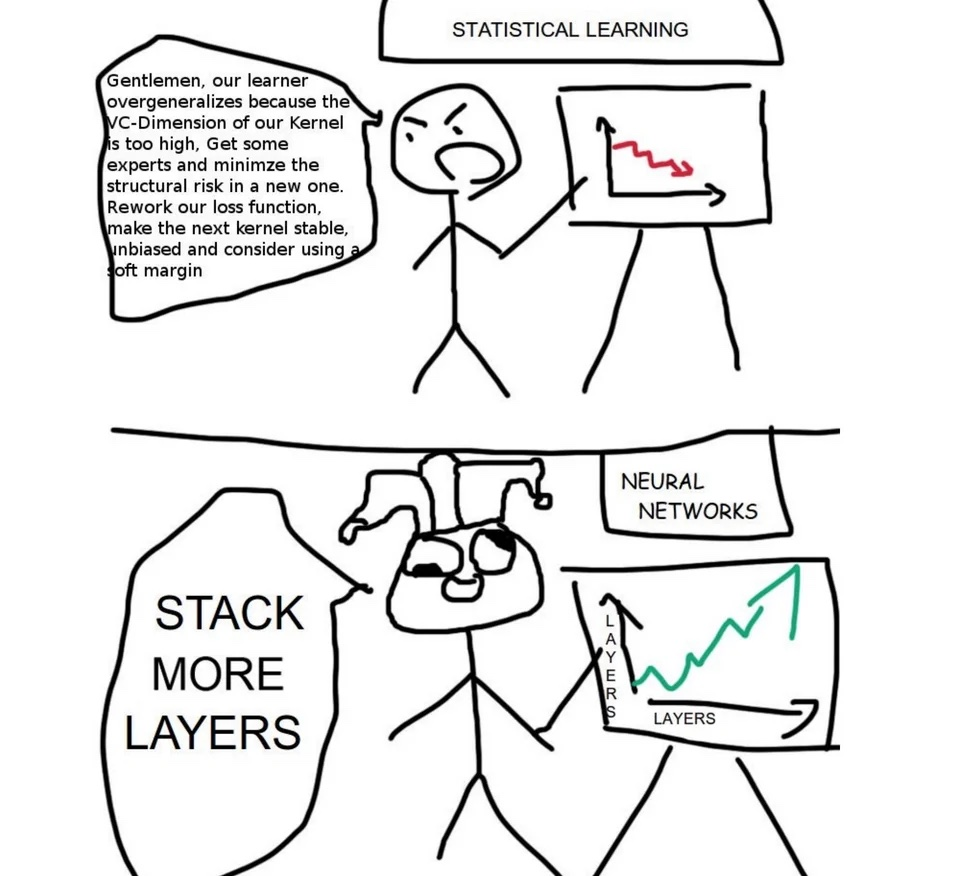
\includegraphics[width=\textwidth]{figures/intro/stackmoar.jpg}
\caption{
A caricature \citep{deleted_user_stack_2018} that summarises the opposing epistemic stances of the symbolic/connectionist divide at a glance. For those unfamiliar, here is a recap. The symbolic side is synonymous with Good-old-fashioned-artificial-intelligence (GOFAI), research programme from the 70s to create general artificial intelligence. However, programming this explicitly turned out to be very hard because it was tantamount to systematising all of reasoning and knowledge \citep{}frameproblem, which is why GOFAI is sometimes described as knowledge-based. In the meantime connectionist methods -- today synonymous with Deep Learning \citep{} -- leapfrogged GOFAI, for reasons explored in more detail in Section \ref{}. What distinguished connectionism was a reliance on data and compute rather than explicit programming, so it is sometimes described as knowledge-lean. A bullish sentiment arose among connectionists that cranking the handle to increase the size of the computer and the amount of training data would suffice to eventually obtain general artificial intelligence \citep{anderson_end_2008}. Debates surrounding this position fall generally under the umbrella of the epistemology of Data Science \citep{pietsch_epistemology_2022,desai_epistemological_2022}. In the case of LLMs specifically, modern debates of the bullish sentiment are developing, often rapidly. For example, in a thorough survey of LLM capabilities, \citep{} warned against a fallacious conflation of linguistic and cognitive abilities, while observing several failure modes of GPT3 in cognitive domains. By the time the paper was published, those observations no longer held for GPT3's successor, ChatGPT \citep{}, which patched the failures with the introduction of reinforcement learning.
}
\end{figure}
 
Connectionism is winning, in the sense that the lion's share of AI research today is connectionist \citep{}. Moreover, hostility (or at least indifference) to symbolic approaches is a stance espoused by some of the leading lights of modern machine learning \citep{}. This stance is worth elaborating and steelmanning for pen-and-paper-people in the context of language. First, many linguistic phenomena are nebulous \citep{} -- the boundary of a simile is like that of a cloud, not sharp like the boundary of a billiard ball. Second, linguistic phenomena are complex, dynamic, and multifactorial: there are so many interacting mechanisms and forces in the production and comprehension of language that even if we do have crisp mathematical models for all the constituent processes we are still left with something computationally irreducible \citep{}. The latter term refers to a special kind of computational difficulty which is best understood by example. We have a closed-form mathematical expression to shortcut the computation of the evolution of a system of two point masses under gravity, but we have no such shortcut for the three-body problem; the best we can do is simulate the system's evolution, and the lesson is that even for very simple systems, it is possible that no amount of causal-mechanistic understanding will simplify compututational simulation. These two points together weakly characterise the kinds of problem domains where machine learning shines. It is just a fact that LLM outputs today conform to any sensible understanding of syntax, semantics, pragmatics, conversational implicature, and whatever else we have theorised. It is just a fact that they produce better poetry and humor than anything we could explicitly program according to our current understanding. It is also a fact that they will only get better from here.\\

So, as far as practical language applications are concerned, the only theories that are nonstarters have to bring something to the table. To borrow terms from concurrency, there is already plenty of liveness, what is needed is more safety; liveness is when the program does something good, and safety is a guarantee it won't do something bad. For example; there is ongoing work in integrating LLMs with stuctured databases for uses where facts and figures matter \citep{}; there is still a need for safeguards to prevent harmful outputs \citep{} and adversarial attacks like prompt injection \citep{}; while LLMs give a very convincing impression of reasoned thought, we would like to be sure if ever we decide to use such a machine for anything more than entertainment, like deciding on a medical course of treatment \citep{} or making decisions with financial consequences \citep{}. The good news is that symbolic-compositional theories are the right shape for safety concerns, because they can be picked apart and reasoned about \citep{}. It is clear however that symbolic-compositional approaches by themselves are nowhere near achieving the kind of liveness LLMs have. Therefore, the direction of progress is synthesis.\\

The core value proposition for synthesis is explainable AI, which operates in a manner we can analyse, and if appropriate, constrain. For this purpose, merely knowing \emph{what} a deep-learning model is thinking is not enough: solving symbol-grounding\footnote{As a contextual aside, I recount the following from \citep{}, which argues that symbol-grounding is solvable from data alone, and in the process surveys the front of the symbol-grounding problem in explainability: the issue of whether LLMs encode what words refer to and mean. On the account of \citep{bender_climbing_2020}, the performance of current LLMs is a form of Chinese Room \citep{searle_minds_1980} phenomenon, so no amount of linguistic competence can be evidence that LLMs solve the symbol-grounding problem -- e.g. knowing what words refer to and mean. However, the available evidence appears to suggest otherwise -- large models converge on word embeddings for geographical place names that are isomorphic to their physical locations \citep{}. Since we know that brain activity patterns encode words in a manner that facilitates analogical reasoning in an abstract conceptual space \citep{}, extrapolating the ability of LLMs to encode analogical representations would in the limit suggest that LLMs encode meanings in a way isomorphic to how we do -- at least for individual tokens.} alone is a necessary but insufficient component. For instance, merely knowing what the weights of subnetworks of an image classification model represent \citep{} does not meet our requirement of an understanding of the computations that manipulate those representations. Moreover, purely data-driven methods to control the computation may incur ethical costs \citep{}, to say nothing of the potential harm that may result from a poorly safeguarded model \citep{}. Add to this the ever-growing dirty laundry lists of AI models failing \citep{} in inhuman ways, and the task of incorporating compositionality -- a formal understanding of \emph{how} models learn and reason -- gains urgency.\\

The investigation of the common ground between symbolic-composition and connectionism takes on, I suggest, essentially two, dual forms. The first kind uses connectionist methods to simulate symbolic-composition. The second kind is the inverse, where connectionist architectures are organised and reasoned with by symbolic-compositional means. Some examples of the first include implementing data structures as operations on high-dimensional vectors, taking advantage of the idiosyncrasies of linear algebra in very high dimension \citep{}, or work that explores how the structure of word-embeddings in latent space encode semantic relationships between tokens \citep{}. Some examples of the second include reasoning about the capability of graph neural networks by identifying their underlying compositional structure \citep{}, or architectures explicitly designed to instantiate symbolic-compositional structures using neural nets as constituent parts, such as GANs \citep{} and gradient boosted decision trees \citep{}. The work in this thesis builds upon a research programme -- DisCoCat, elaborated in Section \ref{} -- which lies somewhere in the middle of the duality. It is, to the best of my knowledge, the only approach that explicitly incorporates mathematically rigourous compositional structures with data-driven learning methods from the ground up. Fortifying this bridge across the aisle requires a little give from both sides; I ask only that reader entertain some pretty string diagrams.

\newthought{\textbf{Objection:} Aren't string diagrams just graphs? We understand graphs well enough that if that were the solution we would have had it by now.}

Yes and no!\footnote{A deeper objection here is that diagrams do not look like serious mathematics. Later I will give ample space to show how they are serious, but the reasons behind this rather common prejudice are worth elaborating. This is the wound Bourbaki has inflicted. Nicolas Bourbaki is a pseudonym for a group of French mathematicians, who wrote a highly influential series of textbooks. It is difficult to overstate their influence. The group was founded in the aftermath of the First World War, around the task of writing a comprehensive and rigourous foundations of mathematics from the ground up. The immediate \emph{raison-d'\^{e}tre} for this project was that extant texts at the time were outdated, and the oral tradition and living history of mathematics in institutions of learning were decimated by the deaths of mathematicians at war. In a broader historical context \citep{}, Bourbaki was a reactionary response to the crisis in the foundations of mathematics at the beginning of the century, elicited by Russell's paradox. Accordingly, their aims were rationalist, totalitarian, and high-modernist \citep{}, favouring abstraction and disdaining visualisation, in line with their contemporary artistic and musical fashions. Consequently, Bourbaki's Definition-Proposition-Theorem style of mathematical exposition is an evolved form of Euclid's that eschews intuition and example, a format pretending at timelessness that requires years of initiation to effectively read and write, and remains \emph{de rigeur} for rigour today in dry mathematics textbooks. The deeper objection arises from the supposition that serious mathematics ought to look arcane and difficult, as most mathematics exposition after Bourbaki is. The reply is that it need not be so, and that it was not always so! The Bourbaki format places emphasis and prestige upon the deductive activity that goes into proving a theorem, displacing other aspects of mathematical activity such as constructions, algorithms, and taxonomisation \citep{}. These latter aspects are better suited for the nebulous subject matter of natural language, which not lend itself well to theorems, but is a happy muse for mathematical play.} This point is best communicated by a mathematical koan. Consider the following game between two players, you and me. There are 9 cards labelled 1 through 9 face up on the table. We take turns taking one of the cards. The winner is whoever first has three cards in hand that sum to 15, and the game is a draw if we have taken all the cards on the table and neither of us have three cards in hand that sum to 15. I will let you go first. Can you guarantee that you won't lose? Can you spell out a winning strategy? If you have never heard this story, give it an honest minute's thought before reading on.\\

The usual response is that you don't know a winning strategy. I claim that you probably do. I claim that even a child knows how to play adeptly. I'll even wager a drink that you have played this game before. The game is Tic-Tac-Toe, also known as Naughts-and-Crosses: it is possible to arrange the cards in a 3-by-3 magic square, such that every column, row, and diagonal sums to 15.\\

The lesson here is that choice of representations matter. In the mathematical context, representations matter because they generalise differently. On the surface, here is an example of two representations of the same platonic mathematical object. However, Tic-Tac-Toe is in the same family as Connect-4 or 5-in-a-row on an unbounded grid, while the game with numbered cards generalises to different variants of Nim. That they coincide in one instance is a fork in the path. In the same way, viewing string diagrams as "just graphs" is taking the wrong path, just as it would be a mistake to dismiss graphs as "just sets of vertices and edges". String diagrams are indeed "just" a special family of graphs, just as much as prime numbers are special integers and analytic functions are special functions.\\

In a broader context, representations matter for the sake of improved human-machine relations. These two representations are the same as far as a computer or a formal symbol-pusher is concerned, but they make world of difference to a human native of meatspace. We ought to swing the pendulum towards incorporating human-friendly representations in language models, so that we may audit those representations for explainability concerns. As it stands, there is something fundamentally inhuman and behavioural about treating the production of language as a string of words drawn from a probability distribution. In practice, this is what large language models (LLMs) do. When \emph{you} use language, do you feel like a diceroll? Even if we grant that the latent space of a data-driven architecture is an analog for the space of internal mental states of a human user of language, how can we know whether the spaces are structurally analogous to the extent that human-machine partnership through the interface of natural language is safe? So here again is the possible solution: we can guarantee that the latent-space representation of the machine is built up in the same way we build up a mental representation when we read a book or watch a film. We sketch how to approach this in Section \ref{}.

\section{\textbf{Question:} How do string diagrams help us understand language better?}

Another way to deal with the first question is to reject it, on the basis that understanding LLMs is completely different from understanding language, and language is worth understanding in its own right. To illustrate this point by a thought experiment, what would linguistics look like if it began today? LLMs would appear to us as oracles; wise, superhumanly capable at language, but inscrutable. Similarly, most people effortlessly use language without a formal understanding which they can express. So the fundamental mystery would remain unchanged. Understanding how an LLM works cannot help: to borrow a thought from \citep{}, suppose you knew the insides of a mechanical calculator by heart. Does that mean you \emph{understand} arithmetic? At best, obliquely: implementing a computer for ideal arithmetic means compromises; the calculator is full of inessentialities and tricks against the constraints of physics. You would not know where the tricks begin and the essence ends. Similarly, suppose you knew every line of code and every piece of data used to train an LLM; does that mean you understand how language works? How could one delineate what is essential to language, and what is accidental? So the value proposition to establish is how string diagrams come into the picture for the linguist. Let's give the practical reader one more objection before we formulate a reply.

\newthought{\textbf{Objection:} If the better theory is one that gives better predictions, aren't many theories of language knocked out of the game by an LLM before they can even get started?}

Whether LLMs are even a theory of language is a best debatable. There are various criteria -- not all independent -- that are arguably necessary for something to qualify as an explanatory theory, and while LLMs satisfice (or even excel) at some, they fail at others. Empirical adequacy -- the ability of theory to account for the available empirical data and make good predictions about future observations -- one such criterion \citep{}, and here LLMs excel. In constast to the idealised and partial nature of formal theories, the nature of LLMs is that they are trained on empirical data about language that captures the friction of the real world. So, in terms of raw predictive power, we should naturally expect the LLMs to have an advantage over principled theories. They are so good at empirical capture that to some degree they automatically satisfy the related criteria of coherence -- consistency with other established linguistic theories -- and scope -- the ability to capture a wide range of phenomena.\\

While empirical capture is necessary for explanatory theories, it is insufficient. We can hold off on vacating linguistics departments when we consider the case study of models of the solar system. The Ptolemaic geocentric model of the solar system was more empirically precise than the heliocentric Copernican, though the latter was "more correct" \citep{}. This was because Ptolemaic epicycles can overfit to approximate any observed trajectory of planets. It took until Einstein's relativity to explain the perihelion of mercury, which at last aligned theoretical understanding with empirical observation. But Newton's theory of gravity was undeniably worthwhile science, even if it was empirically outperformed by its contemporaries.\\

There are several criteria where the adequacy of LLMs is unclear or debatable. Fruitfulness is a sociological criterion for goodness of explanatory theories, in that they should generate new predictions and lead to further discoveries and research \citep{}. While they are certainly a potent catalyst for research in machine learning, it is unclear how they relate to the subject matter of linguistics. Whether they satisfy Popper's criterion of falsifiability is as of yet not determined, because it is not settled how to go about falsifying the predictions of LLMs. The closest examples to falsifiability that come to mind are tests of LLM fallibility for reasoning and compositional phenomena \citep{}, or their weakness to adversarial prompt-injections \citep{}, but these weaknesses do not shed light on their linguistic competence and "understanding" directly.\\

Now the disappointments. LLMs are far from simple, and simplicity (Occam's Razor) is an ancient criterion for the goodness of explanation. Moreover, they fail at providing explanatory mechanisms \citep{}, and they do not unify or subsume our prior understandings \citep{}. The first two points are unobjectionable, so I will briefly elaborate on unification and subsumption of prior understandings, borrowing a framework from cognitive neuroscience. A common methodology for investigating cognitive systems is Marr's 3 levels \citep{} (poorly named, since they are not hierarchical, but more like interacting domains.) Level 1 is the computational theory, an extensional perspective that concerns tasks and functions: at this level on asks what the contents and aims of a system are, to evaluate what the system is computing and why, respectively. Level 2 is representation and algorithm, an intensional perspective that concerns the representational format of the contents within the system, and the procedures by which they are manipulated to arrive at outcomes and outputs. Level 3 is hardware, which concerns the mechanical execution of the system, as gears in a mechanical calculutor or as values, reads, and writes in computer memory. To be fair, in the case of LLMs, we understand well the nature of computational theory level, at least in their current incarnation as next-token-predictors, which is a narrow and clear task. Furthermore, we understand the hardware level well, from the silicon going up through the ladder of abstraction to software libraries and the componentwise activity of neural nets. There is something deeply wrong about our understanding -- if we can call it that -- of level 2. We have working understandings of several aspects about this level. We know something about the nature of internal representations in neural nets both in terms of semantic encoding within weight distributions \citep{} and of token-embeddings in latent space \citep{}. We can explain how transformer models work in terms of attention mechanisms and lookback \citep{}, which serves as working understanding of the procedural aspect of LLMs. We also understand mathematically how it is that these models are trained using data to produce the outputs they do. The deep problem is that in spite of these understandings which should jointly cover all of level 2, we only obtain explanations at the wrong level of abstraction for the purposes we care about \citep{}. Level 2 is in a sense the important level to get right for the purposes of explainability, auditability, and extension, since it is at the level of representation and procedure that we can investigate internal structure and match levels of abstraction across domains. Since the three levels interact, the challenge is to slot in a story about level 2 that coheres with what we already know about levels 1 and 3, and this is a core philosophical aim of string diagrams in general, and text circuits in particular.

\newthought{\textbf{Reply:} String diagrams are a good metalanguage for formal linguistics}

Set-theoretical foundations of mathematics are not well suited for complex and interacting moving parts. The chief drawback is that if you want to specify a function, you have to spell out how it behaves on the domain and codomain, which means spelling out what the innards of the domain and codomain are; to specify a set-theoretic model necessitates providing complete detail of how every part looks on the inside\footnote{This is a foundational, innate problem of set theory. Consider the case of the cartesian product of sets, one of the basic constructions. $A \times B$ is the "set of ordered pairs" $(a,b)$ of elements from the respective sets, but there are many ways of encoding that are equivalent in spirit but not in syntax; a sign that the syntax is a hindrance. What we really want of the product is the property that $(a,b) = (c,d)$ just when $a = c$ and $b = d$. Now here is a small sampling of different ways to encode an ordered pair. Kuratowski's definition is
\[A \times B := \bigg\{ \{\{a\},\{a,b\}\} \ | \ a \in A \ , \ b \in B \bigg\}\]
Which could have just as easily been:
\[A \times B := \bigg\{ \{a,\{a,b\}\} \ | \ a \in A \ , \ b \in B \bigg\}\]
And here is Wiener's definition:
\[A \times B := \bigg\{ \{\{a,\varnothing\},b\} \ | \ a \in A \ , \ b \in B \bigg\}\]}. As you may be familiar with, this representation-dependency is a nightmare when dealing with a complex system: you have to specify all the implementation details from start to finish, bottom-up. This leads to at least three problems.
\begin{enumerate}
\item{
The sociological problem is that this makes things difficult to understand unless you have invested a lot of time into mathematics in general.
}
\item{
Interoperability is tricky. When a programmer wants to use a data structure or algorithm, they do not always write it from scratch or copy code from stackoverflow; they may use a library that provides them structures and methods they can call without worrying about how those structures and methods are implemented all the way down. However, if you building a complex theory by spelling out implementations set-theoretically from the start, incorporating a new module from elsewhere becomes difficult if that module has encoded things in sets differently. A lot of busywork goes into translating foundations of formalisms at an analogous level to machine code, which is time better spent building upwards and outwards. A computer scientist might say that some abstraction is needed, and being one, I say so.
}
\item{
Third, and related to the second, is that set-theory is not the native language for the vast majority of practical computation. Often in the design of complex theories, we do not care about how precisely representations are implemented, instead we only care about placing constraints or guarantees on the behaviour of interacting interactions -- that is, we care about operational semantics.
}
\end{enumerate}

The problems I have mentioned above are obstacles, and I hope to show that using applied category theory as a metalanguage may be a solution. A broad theme of this thesis is to illustrate the economy and reach of applied category theory for dealing with compositional phenomena. Our capacity for language is one of the oldest and sophisticated pieces of compositional technology, maybe even the foundation of compositional thought. So, linguists are veteran students of compositionality and modularity. How does syntax compose meaning? How do the constraints and affordances of language interact? The discipline embodies a encyclopaedic record of how compositionality works "in the field", just as botanists record flowers, early astronomers the planetary motions, or stamp collectors stamps. But a disparate collection of observations does not a theory make; we will inevitably wish to bring it all together. I show that we can progress towards this aim using formal diagrams that our visual cortexes have built-in rules to manipulate, and that allow us to work at the level of abstraction we choose, so that we may easily incorporate other modules and find implementations in a variety of settings.\\

To summarise the core value proposition, string diagrams are an aesthetic, intuitive, flexible, and rigourous metalanguage syntax that gives agency to the modeller by operating at a level of abstraction of their choice. This means that the same diagrams are a common syntactic foundation that can model linear and affine algebra \citep{}, first order logic \citep{}, signal flow \citep{}, electrical circuits \citep{}, database operations \citep{}, spatial relations \citep{}, language games \citep{}, petri nets \citep{}, hypergraphs \citep{}, probability theory \citep{}, machine learning \citep{}, and quantum theory \citep{}, to name just a sample. In this vein, theories of syntax expressed in terms of string diagrams makes it easier to reason about expressive equivalence between theories at a compositional level. More precisely, a theory of syntax is expressed as a finitely presented symmetric monoidal category, and relationships between theories are expressed as symmetric monoidal functors, which are generalised structure-preserving maps. The upshot of reasoning in this way is that equivalences are established at a structural level between the atomic components of corresponding theories, which lets us do some crazy things. Demonstrating all this constitutes the rest of the thesis, so let's see an itinerary.

\section{Synopsis of the thesis}

\marginnote{
\textbf{Novel contributions:}
\begin{itemize}
\item
Section \ref{} demonstrates how string-diagrammatic reasoning allows for graphical proofs of strong equivalences between typelogical, string-production, and further strong equivalence to a fragment of tree-adjoining grammars. 
\item
Text diagrams and text circuits lie at the heart of the above correspondences and of this thesis, which we introduce and investigate in Section \ref{} in an abridged re-presentation of \citep{}, culminating in a proof relating the expressive capacity of text circuits to a controlled fragment of English that serves as evidence that text circuits are a natural metalanguage for grammatical relationships that make no extraneous distinctions.
\item
In Section \ref{}, moving towards applications, I introduce the category of continuous relations, to set a mathematical stage upon which we can build toy models, expanding upon my previous work on linguistically compositional spatial relations \citep{} towards modelling mechanical systems and containers.
\item
I mathematically investigate the possibilities and limitations of textual modelling with text circuits on classical and quantum computers in Section \ref{} by examining the limitations of cartesian monoidal categories for modelling text circuits, taking the universal approximation theorem into account.
\item
In Section \ref{}, I extend the string-diagrammatic techniques used to prove correspondences between different syntactic theories to text circuits provides a framework for the formal, conceptually-compliant modelling of textual metaphor.
\item
I demonstrate a formal connection between tame topologies and tensed language in Section \ref{}, which extends to a formal framework to model narratives as database rewrites in Section \ref{}.
\end{itemize}
}

Chapter 2 provides the relevant background and foundations for category theory, machine learning, and formal syntax for this thesis, which lives at the intersection. The ideas required from the parent fields will be basic, so the exposition is meant to get readers across disciplines on the same page, not impress experts. For string diagrams I will first provide a primer for how process-theoretic reasoning with string diagrams work, by example. On the category theoretic end, I will recount symmetric monoidal categories as the mathematical objects that string diagrams are syntax for, as well as provide a working understanding of PROPs \citep{} and n-categories as formalised by \citep{}, which provide a metalanguage for specifying families of string diagrams. Once the reader is happy with string diagrams, for machine learning I will just introduce how deep neural nets and backpropagation work in string-diagrammatic terms to provide a foundation of formal understanding, and I will explain the mathematical and real-world reasons why deep learning is so powerful. For formal linguistics, I will sketch out a partial history of categorial linguistics in general, along the way briefly recasting \citep{} in more modern mathematical terminology to justify string diagrams as a generalisation of Montague's original conception of syntax and semantics. Once all of this context is in place, I will introduce DisCoCirc, make it stand trial against charges of inadequacy, sentence it to death, and replace it with something better.\\

Chapter 3 is about string diagrams for formal syntax. Here I recount context-free, pregroup, and tree-adjoining grammars to the reader, recast them string-diagrammatically, and relate them by means of discrete monoidal fibrations, a piece of mathematics I will develop. Then we (re)introduce text circuits as the common structure between those different theories of grammar that abstracts away differences in linear syntactic presentation while conserving a core set of grammatical relations. During my DPhil, I wrote a paper \citep{} in collaboration with Jonathon Liu and Bob Coecke which introduced text circuits in a pedestrian way, and characterised their expressive capacity with respect to a controlled fragment of English. To avoid reproducing too much, here I will only reproduce the main beats of that paper, the proof of the characterisation theorem, and examples to demonstrate how language beyond the controlled fragment may be treated as text circuits.\\

Chapter 4 sets the mathematical stage for us to model and calculate using text circuits. I introduce the category of continuous relations \textbf{ContRel}, a na\"{i}ve generalisation of the category of continuous maps between topological spaces which I introduce for the sake of having a sufficiently expressive and cognitively motivated concrete mathematical domain in which to interpret and calculate with text circuits. For category theorists, I demonstrate that the categorically obvious approaches to obtaining such a category either do not work or yield something different. The central theorem in this section is a diagrammatic characterisation result which establishes that a generalisation of special frobenius algebras in \textbf{ContRel} provide formal semantics for the kinds of schematic doodle cartoons we might draw on paper to illustrate events occurring in space.\\

Chapter 5 is about formal semantics beyond Montague and logic that text circuits in \textbf{ContRel} allow us to explore. I model generalised anaphora that reference any meaningful part of text; I provide formal semantics for the container metaphor in particular and textual metaphors in general; I sketch a formal correspondence between tensed language and tame topologies that extends to formally reckoning with narrative structure. I am not interested in whether these topics have been mathematicised more thoroughly and deeply before; what I care to demonstrate is that diagrammatic reasoning and some imagination can go a long way.\\

Finally, I close with a discussion and prospectus. For the convenience of the reader, bibliographies are placed at the end of each chapter. I hope you enjoy the read, or if nothing else, I hope you like my diagrams!
